
%%%%%%%%%%%%%%%%%%%%%%%%%%%%%%%%%%%%%%%%%%%%%%%%%%%%%%%%%%%%%%%%%%%%%%%%%%%%%
%
%  System        : 
%  Module        : 
%  Object Name   : $RCSfile$
%  Revision      : $Revision$
%  Date          : $Date$
%  Author        : $Author$
%  Created By    : Jim Finnis
%  Created       : Mon Oct 4 09:50:39 2010
%  Last Modified : <150408.1206>
%
%  Description 
%
%  Notes
%
%  History
% 
%%%%%%%%%%%%%%%%%%%%%%%%%%%%%%%%%%%%%%%%%%%%%%%%%%%%%%%%%%%%%%%%%%%%%%%%%%%%%
%
% Copyright (c) 2010 Jim Finnis.
% 
% All Rights Reserved.
% 
% This  document  may  not, in  whole  or in  part, be  copied,  photocopied,
% reproduced,  translated,  or  reduced to any  electronic  medium or machine
% readable form without prior written consent from Jim Finnis.
%
%%%%%%%%%%%%%%%%%%%%%%%%%%%%%%%%%%%%%%%%%%%%%%%%%%%%%%%%%%%%%%%%%%%%%%%%%%%%%

\documentclass[a4paper]{article}
\usepackage{wrapfig}
\usepackage[pdftex]{graphicx}
%\usepackage[version=3]{mhchem}
\usepackage{fancyvrb}
\usepackage{multirow}
\usepackage{url}
\usepackage{amssymb}
\usepackage{enumitem}

\usepackage[hmargin=2.5cm,vmargin=3.5cm]{geometry}
\usepackage{multicol}
% In math mode, put a word into text inside anglebrackets. Used for BNF, sometimes.
\newcommand{\angb}[1]{\text{$<$\\#1$>$}}

% so we can do 3\e{4} to do 3x10^4
\providecommand{\e}[1]{\ensuremath{\times 10^{#1}}}


\newenvironment{prettycode}
{\begin{quote}\ttfamily\small}
{\end{quote}}

\DefineVerbatimEnvironment{v}{Verbatim}{
    %numbers=left,numbersep=5pt,
    %frame=lines,framerule=0.5mm,
    fontsize=\small,xleftmargin=15pt}
\DefineVerbatimEnvironment{vv}{Verbatim}{
    %numbers=left,numbersep=5pt,
    %frame=lines,framerule=0.5mm,
    fontsize=\small,xleftmargin=15pt}
\DefineVerbatimEnvironment{v2}{Verbatim}{
    %numbers=left,numbersep=5pt,
    %frame=lines,framerule=0.5mm,
    fontsize=\scriptsize,xleftmargin=0pt}
\DefineVerbatimEnvironment{v3}{Verbatim}{
    %numbers=left,numbersep=5pt,
    %frame=lines,framerule=0.5mm,
    fontsize=\tiny,xleftmargin=0pt}
\DefineVerbatimEnvironment{bv2}{BVerbatim}{
    %numbers=left,numbersep=5pt,
    %frame=lines,framerule=0.5mm,
    fontsize=\scriptsize,xleftmargin=0pt}
\DefineVerbatimEnvironment{bv}{BVerbatim}{
    %numbers=left,numbersep=5pt,
    %frame=lines,framerule=0.5mm,
    fontsize=\scriptsize,xleftmargin=0pt}
\DefineVerbatimEnvironment{bvc}{BVerbatim}{
    %numbers=left,numbersep=5pt,
    %frame=lines,framerule=0.5mm
    commandchars=+\[\],
    fontsize=\scriptsize,xleftmargin=0pt}

\setcounter{secnumdepth}{5}
\setcounter{tocdepth}{5}

\title{Blodwen rover documentation}
\date{\today}
\author{James Finnis, jcf1@aber.ac.uk}

\begin{document}
\maketitle
\newpage
\tableofcontents

\newcommand{\isqc}{$\mathrm{I}^2\mathrm{C}$}

\newcommand{\todo}[1]{
    \begin{center}
    \fbox{\parbox{4in}{\textbf{To Do}\vspace*{1em} \\#1}}
    \end{center}}

\newcommand{\boxy}[1]{
    \begin{center}
    \fbox{\parbox{4in}{#1}}
    \end{center}}
    
% level 2 lists are normally indicated by dashes - I'm changing this
% because it looks too much like a minus sign.
\renewcommand{\labelitemii}{$\circ$}

\subsection{Checklists}
Much of this data is repeated in more detail later in the document,
which should be read before use (at least up to and including section~\ref{angcont}).
\subsection{Rover startup checklist}
\begin{enumerate}
\item Ensure the battery inside the main compartment is charged.
\item Ensure main compartment lid is closed.
\item Switch on PCs using the PC power button.
\item If it's installed, you may wish to switch off the science PC (the right-hand PC). The button is on
the front of the PC, near the floor of the compartment.
\item Check current is less than 2A.
\item Connect a laptop to the rover's WiFi network (the SSID contains ``EnGenius'').
\item SSH into the rover: host 192.168.0.10, username \emph{blodwen}, password \emph{robotics}.
\item Switch on the motors with the other power switch on the lid.
\item Check that the underside lights go steady on, then flash at about 1Hz.
\item Check current is about 1.8 to 2A.
\item (The list from here implies direct rover control via Angort)
\item In the terminal SSHing into the rover, issue the commands
\begin{v}
cd r
./rover
\end{v}
\item Ensure the connection is made --- \texttt{READY} should appear
and the Angort prompt \texttt{1|0>}.
\item Issue the commands
\begin{v}
reset calib
\end{v}
to reset the initial boot exception state and send calibration data.
\item Now refer to section~\ref{angcont} for commands.
\item In the case of an emergency, hammer CTRL-D (or CTRL-C if that
fails) to send an emergency stop. All gains will be zeroed, and 
\texttt{reset calib} must be reissued to restart the rover.
\end{enumerate}
\subsection{Rover shutdown checklist}
\begin{enumerate}
\item Exit the Angort interpreter with CTRL-D or \texttt{quit}.
\item Switch off the motors.
\item Power down the locomotion PC with \texttt{sudo poweroff}.
\item Wait for the power consumption to drop to about 1A (indicating
PC powerdown).
\item Switch off the PC power using the other power switch.
\end{enumerate}



\section{Introduction}
The rover's control architecture consists of three layers, as shown
in figure~\ref{fig1}:
\begin{description}
\item[A PC running the main control software] which is interfaced to the
hardware via a register interface. It sends register read/write commands
to the Arduino. In many situations, this control layer will itself
be a server responding to commands sent by another system.
\item[An Arduino accepting register read/write commands] which passes
them over
\isqc{} to nine motor controllers. This is referred to in the text as
the \textbf{master controller.} It also has a set of registers of its own
for global system information.
\item[Nine motor controller boards]\footnote{Sparkfun ``serial controlled
motor driver'' boards, ROB-09571} each containing an ATMega328p processor
(effectively an Arduino) to handle the PI control algorithms and respond
to register read/write commands for two motors, using an
L298P dual H-bridge to drive the motors. Each board may also have an analogue
input for the chassis potentiometer.

These are
referred to in the text as \textbf{slave} or \textbf{secondary controllers.} 
\end{description}

\begin{figure}[ht]
\center
\includegraphics[width=6in]{fig1.pdf}
\caption{Overall architecture}
\label{fig1}
\end{figure}

All software is written in C++, with the both master and slave controller
code being written in the Arduino variant, burned directly into the chip
using ICSP.

\subsection{Wheel pair architecture}
\label{whpairarc}
The rover has six wheels, each pair of which is controlled by three
slave controllers as shown in figure~\ref{fig2}.
This shows that there are two distinct kinds of slave controllers:


\begin{figure}[ht]
\center
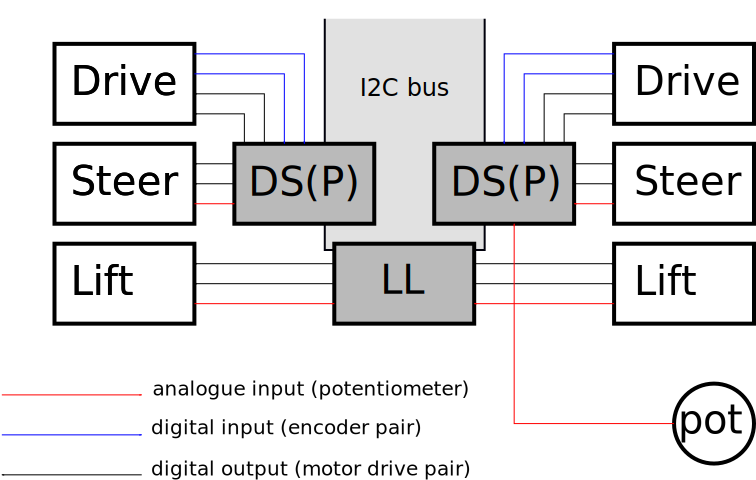
\includegraphics[width=4in]{hardwareoverview.pdf}
\caption{Hardware overview of a single wheel pair}
\label{fig2}
\end{figure}

\begin{description}
\item [Two Drive/Steer/(Position) controllers per pair,] which each control the driving
and steer motor on one wheel. One of these also receives an input from
one of the three chassis configuration potentiometers. On the other, this
input is ignored.
\item [One Lift/Lift controller per pair,] which control the lift motors on both wheels.
\end{description}
The reason for this split is that each controller board can only handle 
two analogue inputs (in addition to the two internal current sensor channels.)

The controllers and the wheels they control are numbered as in figure~\ref{fig3}.
The wheel numbering scheme is that given in the rover documentation.

\begin{figure}[ht]
\center
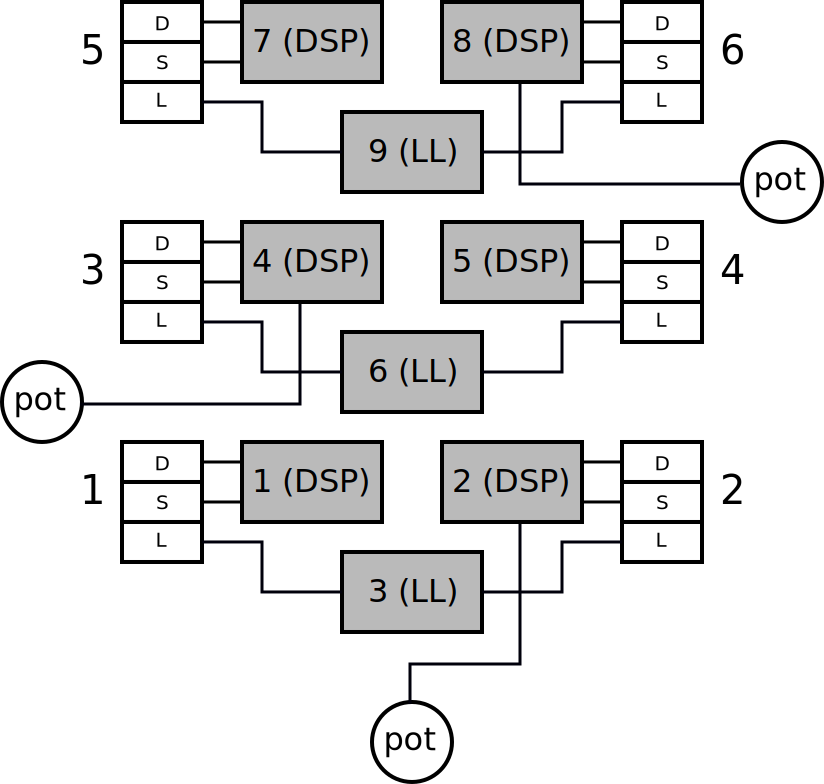
\includegraphics[width=4in]{numbering.pdf}
\caption{Numbering of controllers and wheels}
\label{fig3}
\end{figure}

\clearpage
\section{Using the rover}
The rover is shown in Figure~\ref{fig:blod}. 
\begin{figure}[ht]
\center
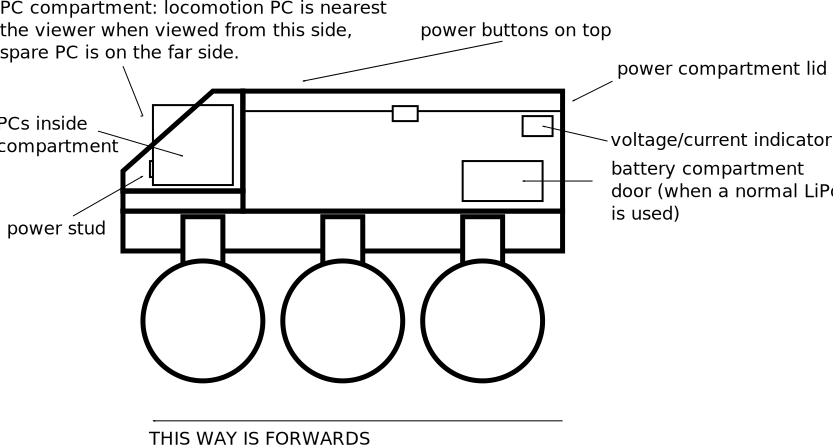
\includegraphics[width=5in]{blod.pdf}
\caption{The Blodwen rover}
\label{fig:blod}
\end{figure}
Note that the rover's ``front'' is the obvious, wedged end.


\begin{itemize}
\item The main compartment contains a LiPo battery suitable for most applications. Ensure this is charged
prior to use.
\item The battery compartment has space for an extra LiPo battery. If you are using this, the connector
needs to be passed through from the main compartment. Ensure you connect with the correct polarity.
\item Switch on the rover PCs by pressing the PC power button on the roof of the chassis.
\textbf{Once this has been done, do not power off the rover without shutting the locomotion PC down from
a terminal connection.}
\item Check that the voltage and current are nominal (11.5-12V, $<3$A) using the indicator. If they are
not, shut down the rover and power off.
\item The PCs are in the wedge-shaped compartment at the front of the rover.
If another PC is in use, switch off the spare PC. This is the PC located on the right side of the rover.
The power studs are located at the bottom of the PC
front panels. Figure~\ref{fig:blod2} shows the arrangement of the PCs more clearly. Power consumption should drop
to $\sim 1.5$A.
\begin{figure}[ht]
\center
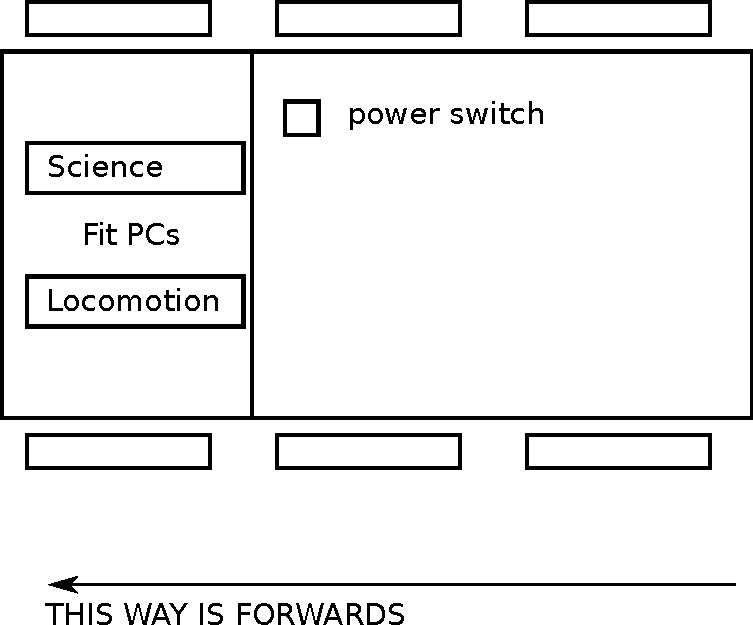
\includegraphics[width=3in]{blod2.pdf}
\caption{The Blodwen rover, from above}
\label{fig:blod2}
\end{figure}
\item To power up the motor, drive and chassis electronics the motor power switch on the lid should be pressed.
\item The lights under the chassis should come on briefly, and then begin to flash approximately
once a second. Power consumption should rise to $\sim 1.8-2$ A. The hardware is now ready to receive commands. Proceed to
section~\ref{angort} to find out how to command it with the Angort language.
\end{itemize}

\subsection{Detailed explanation of LED flashes}
This guide may help diagnose wiring problems inside the rover chassis:
\begin{itemize}
\item Each controller has two LEDs. As the rover boots, each controller
should show the lowest 2 bits of its \isqc{} address (1-9) on the LEDs
for about half a second. This causes the initial lighting state.
\item The master and slaves will start in the boot exception state,
so the LEDs will be steady on. Shortly after boot, the master will attempt to send
resets to each slave. 
\item If the send fails, the \isqc{} bus will hang, so the master's
watchdog timer will time out and the master will reboot and try again. A
common failure mode is repeated reboot cycles, where the the good slaves
are resetting successfully from the boot exception, shown by repeated off
gaps, while the bad slave will just show a steady exception state (see
below).
\item If the slaves all reset successfully, the master will receive
the acknowledgements and begin awaiting PC packets. It will also
send a ``ping'' message to the slaves once per second. If a slave receives
this, it will briefly flash an LED (LED1 on a drive/steer unit,
LED2 on a lift/lift unit). Therefore, the LEDs should flicker once per
second on all slaves once the rover is ready to receive commands.
\end{itemize}

In the exception state, the two LEDs will stay on showing:
\begin{itemize}
\item LED1: motor 1 is in exception
\item LED2: motor 2 is in exception
\item both LEDs: the exception is not a motor exception
\end{itemize}

\subsubsection{Using the remote control}
\textbf{(Note: this hasn't been tested for a while).}
Turning on the remote control causes the master's main loop to ignore any
instructions sent from the PC, and also recalibrates the rover (i.e. a new
set of PID and extent parameters will be sent). Therefore, the rover will
need to be recalibrated (by calling the \textbf{calibrate()} method) if
PC control is desired again.

When the remote control is active, a blue LED should shine under the rover,
clearly visible on the driving surface. The controls are as follows:
\begin{itemize}
\item Left stick forward/backward : drive speed
\item Right stick left/right: turn steer wheels
\item Right stick forward: alternate steer mode
\end{itemize}
By default, steering operates using Ackermann steering on the front
and back wheel pairs in opposite directions, with the centre wheels not commanded.
If the right stick is pushed forwards to its limit, the same steering angle
will be applied to all wheels, permitting ``crabbing''.

\subsection{Controlling the rover with Angort}
\label{angort}
The rover locomotion PC has the language Angort installed, with a set of scripts and native C++ word
definitions to allow easy control. To run the language interpreter, one must connect to the locomotion
PC via SSH. Both PCs are connected to a WiFi router installed inside the rover.

\subsubsection{Connecting to the rover and starting Angort}
\begin{itemize}
\item Power up the rover. Power down the science/spare PC immediately (see above).
\item Connect to the rover on the EnGenius router via SSH (IP address 192.168.0.10, username
\textbf{blodwen}, password \textbf{robotics}).
\item \texttt{cd r} to get into the appropriate directory (this is a soft link to a subdirectory).
\item Power on the electronics by closing the battery door.
\item \texttt{./rover} to start a special version of the Angort interpreter with rover control words
added. The script \texttt{script.ang} will automatically
be loaded --- it contains a useful set of word definitions to enhance those built in.
\item A few lines should show the connection to the master Arduino being established, and initial rover library setup. 
The Angort prompt
\begin{v}
1|0 >
\end{v}
should appear (the left number is the number of GC-objects in the system, the right number is
the depth of the stack). If this initial connection phase fails, check that the safety switches are
closed and that the microcontrollers are all flashing as they should.
\end{itemize}

\subsubsection{Rover control commands}
\label{angcont}
The rover boots in an exception state as a safety feature, and also has all PID gains in the motors
set to zero. Before it can move, all the controllers need to have their exceptions reset, and correct
PID gains uploaded. To do this, issue the following commands \textbf{but be prepared to hammer CTRL-D}:
\begin{v}
reset calib
\end{v}
This may result in some small motion of the wheels if the rover has been moved by hand or is
in an unusual configuration for some other reason. \textbf{If the motion is dangerous, hit CTRL-D} to
reset the system.

Once this has been done, movement commands may be issued. If they appear to do nothing, check
that \texttt{reset} and \texttt{calib} have been run.
The following table shows examples of the most common commands for controlling the rover:

\begin{tabular}{|l|p{4in}|} \hline  
\texttt{1000 d} & \textbf{set all drive motors to speed 1000} forwards, towards the wedged end with the PCs.\\
\texttt{-2500 d} & \textbf{set all drive motors to speed -2500}, i.e. backwards --- note that 2500 is about the highest safe speed.\\
\texttt{40 t} & \textbf{turn $40^\circ$,} done by setting the front steer wheels to the given angle and the rear wheels to
the opposite.\\
\texttt{-40 t} & \textbf{turn the opposite way} to the previous command.\\
\texttt{40 a} & \textbf{set all steer motors to $40^\circ$,} useful for ``crabbing''.\\
\texttt{20 setliftall} & \textbf{set all lift motors} to $20^\circ$.\\
\texttt{20 1!lift} & \textbf{set lift lift motor 1} to $20^\circ$. The notation
\begin{v}
<value> <motornumber>!<motortype>
\end{v}
can be used to set individual drive, steer and lift motor speeds and positions. \textbf{Be careful} ---
it's possible to make the rover perform potentially damaging actions by setting individual motors.\\
\texttt{1?lift.} & \textbf{get and print the requested position for lift motor 1.}
\\ \hline
\end{tabular}

\subsection{Monitoring the rover graphically}
The Angort scripting system, once connected to the rover hardware, constantly sends a stream of key/value
pairs over UDP to port 13231 on host 192.168.0.100 (the first router address available to WiFi hosts). 
The \texttt{monitor} program can read this data and display it graphically with an appropriate configuration
file.

The program is available at \url{https://github.com/jimfinnis/monitor.git} and is a Qt4 application. It
requires the \texttt{libmarblewidget} library to compile (adding support for mapping; the monitor
is also used for robotic boat trials). A suitable configuration file is provided --- once compiled, run
the program with
\begin{v}
monitor -f ./roverconfig
\end{v}
This configuration will display the desired and actual drive motor speeds, the actual lift and
steer positions, the current readings for the 6 drive wheel controllers, the temperatures of all
9 controllers above ambient. Extra variables are shown for hormone settings and traversed distance,
but these are provided by code built for particular experiments beyond the scope of this document.

\section{Hardware details}
The hardware is implemented as three motherboards, onto each of which are mounted
three motor controller daughterboards. Each motherboard controls one
pair of motors. Screw connectors on the board connect the motors, potentiometers
and encoders; also the \isqc{} and power busses.

A circuit diagram and PCB layout for a single board can be found in the \emph{eagle} directory.

Each controller daughterboard has a unique \isqc{} address, which is set
as a parameter of the \emph{upload} script. 

\subsection{Procedure for updating the master firmware}
Ino (\verb+www.inotool.com+) must be installed to build the firmware, which
is then uploaded over the USB connection:
\begin{v}
cd rover/firmware/master
(edit code)
ino build
./upload
\end{v}
\subsection{Procedure for updating the slave firmware}
Ino (\verb+www.inotool.com+) must be installed to build the firmware, which
is then uploaded using a USBTiny ICSP programmer:
\begin{v}
cd rover/firmware/slave
(edit code)
\end{v}
and then either
\begin{v}
./blift
\end{v}
to build firmware for a lift/lift controller, or
\begin{v}
./bdrive
\end{v}
to build firmware for a drive/drive controller.
Then connect the ICSP to the controller and run
\begin{v}
./upload N
\end{v}
where $N$ is the controller number. It is possible to upload the software
to several different controllers without rebuilding it:
\begin{v}
./blift
./upload 3
./upload 6
./upload 9
./bdrive
./upload 1
./upload 2
./upload 4
./upload 5
./upload 7
./upload 8
\end{v}
is a typical scenario. Of course, you'll have to plug the programmer
onto the ICSP pins for the each board for each command.


\subsection{Pullup resistors}
Note that the \isqc{} internal pullup resistors are disabled on all
the microcontrollers. Therefore a pair of pullups of a suitable
value are added, pulling up to 3V. These are on a shield board mounted
onto the Arduino, along with an additional pullup for the OneWire bus
managing the temperature sensors.

\subsection{Controller assignments}
Figure~\ref{fig3} shows the controller/wheel assignments. For example,
the steer and drive wheel of controller 1 is wheel number 5, while
controller 3 controls the lift motors on wheels 5 and 6.

\subsection{Connections}
The following connections are used on the master:
\begin{itemize}
\item \textbf{USB} connection for control
\item \textbf{A4} for \isqc{} SDA line
\item \textbf{A5} for \isqc{} SCL line
\end{itemize}
The following connections are used on the DS(P) slaves:
\begin{itemize}
\item \textbf{M1+/M1-} for drive motor
\item \textbf{M2+/M2-} for steer motor
\item \textbf{ADC6} for steer potentiometer
\item \textbf{ADC7} for chassis potentiometer if present
\item \textbf{TX} for drive motor encoder channel A
\item \textbf{RX} for drive motor encoder channel B
\end{itemize}
The following connections are used on the LL slaves:
\begin{itemize}
\item \textbf{M1+/M1-} for lift motor 1
\item \textbf{M2+/M2-} for lift motor 2
\item \textbf{ADC6} for lift potentiometer 1
\item \textbf{ADC7} for lift potentiometer 2
\end{itemize}
The layout of a single board is shown in figure~\ref{boardfig}, while
the layout of all the boards inside the body of the rover is shown in
figure~\ref{internalwiring}.

\begin{figure}[ht]
\center
\includegraphics[width=3in]{boardDrawing.pdf}
\caption{Board connections}
\label{boardfig}
\end{figure}

\begin{figure}[ht]
\center
\includegraphics[width=5in]{internalWiring.pdf}
\caption{Internal layout of the main rover compartment}
\label{internalwiring}
\end{figure}

\clearpage
\subsubsection{Connection labelling}
Wires running to the motors --- both sensor and motor control wires ---
are marked using coloured rings of insulation.
Figures \ref{senscols} and \ref{motorcols} show the schemata used.
Note that in both diagrams, the proximal (motor controller board) end is shown to the
right.

\begin{figure}[ht]
\center
\includegraphics[width=5in]{sensors1.pdf}
\caption{Sensor wire labelling scheme}
\label{senscols}
\end{figure}


\begin{figure}[ht]
\center
\includegraphics[width=5in]{motors1.pdf}
\caption{Motor wire labelling scheme}
\label{motorcols}
\end{figure}

Other colours:
\begin{itemize}
\item \isqc{} bus : blue and white twisted pair --- the white line is the SDA, the
blue line is SCL.
\item Power bus : black and red twisted pair --- red is +12V, black is ground
\item Power input : brown is +12V, green/yellow is ground
\item OneWire bus : orange and orange/white twisted pair --- orange is ground,
orange/white is data
\item Chassis lines: red is +5V, black is ground, yellow is data. There's
no ID marking; the line can be clearly traced to its potentiometer by eye.
\end{itemize}
\clearpage
\subsection{Remote control connections}
The remote control is connected to the master Arduino Uno as shown in
figure~\ref{fig:remo}.
\begin{figure}[ht]
\center

\includegraphics[width=4in]{remote.pdf}
\caption{Servo receiver connections}
\label{fig:remo}
\end{figure}



%%%%%%%%%%%%%%%%%%%%%%%%%%%%%%%%%%%%%%%%%%%%%%%%%%%%%%%%%%%%%%%%%%%%%%%%%%%%%
%
%  System        : 
%  Module        : 
%  Object Name   : $RCSfile$
%  Revision      : $Revision$
%  Date          : $Date$
%  Author        : $Author$
%  Created By    : Jim Finnis
%  Created       : Mon Dec 10 22:01:02 2012
%  Last Modified : <130605.1035>
%
%  Description 
%
%  Notes
%
%  History
% 
%%%%%%%%%%%%%%%%%%%%%%%%%%%%%%%%%%%%%%%%%%%%%%%%%%%%%%%%%%%%%%%%%%%%%%%%%%%%%
%
% Copyright (c) 2012 Jim Finnis.
% 
% All Rights Reserved.
% 
% This  document  may  not, in  whole  or in  part, be  copied,  photocopied,
% reproduced,  translated,  or  reduced to any  electronic  medium or machine
% readable form without prior written consent from Jim Finnis.
%
%%%%%%%%%%%%%%%%%%%%%%%%%%%%%%%%%%%%%%%%%%%%%%%%%%%%%%%%%%%%%%%%%%%%%%%%%%%%%

\section{Onboard PC library}
The onboard PC currently uses a library of C++ classes to abstract
the communications protocol, the details of \isqc{}, and
the vagaries of the firmware register set (for the reasons given
in section~\ref{firmrec}, working out which slave controller to send
commands to in order to turn a particular wheel is not straightforward.)

This section contains a brief overview of the C++ classes, describing their
functions but not going into any details of methods.


\subsection{Rover}
The \emph{Rover} class is the top-level class. The utilising code is expected
to instantiate a single object of this class. Calling the initialisation method
\emph{init} 
with a character device name and a baud rate will start a connection to the master
controller (the Arduino) which will be reset. Once the connection is made,
calling \emph{update} periodically will request state information about all the 
devices.

Other methods allow the user access to motor objects, which will allow the user
to change motor parameters and required speeds/positions; and to motor data
blocks, allowing users to monitor the motors. The data blocks will contain
information received at the last \emph{update.} 

Note that the communications over \isqc{} have been kept to a minimum --- the
rover uses the ``set read set'' firmware protocol command (see
section~\ref{protoc}) to send a set of registers. When a simple 3 byte ``read
set'' command is set with a set number, the slave will send a packet of all
the registers in that set.

Internally, the rover uses the \emph{WheelPair} class to manage triplets
of slave controller boards, which in turn use \emph{MotorDriverData} objects
to manage reading data from the two types of slave (the \emph{Motor} class
handles writing values.) 

Communications are handled by \emph{SlaveProtocol}, which in turn uses
\emph{SerialComms.} 

\subsection{Motor}
This class contains methods to send parameters (such as PID gains) to a motor,
set its required position or speed, and reset any exception condition\footnote{for example, if
a motor's current exceeds its overcurrent threshold, the slave will detect this
and shut the motor down.}. There are three subclasses of \emph{Motor}, one
for each motor type: \emph{DriveMotor}, \emph{SteerMotor} and \emph{LiftMotor.} They present similar interfaces to the user.
Pointers to motor objects can be obtained by calling methods in \emph{Rover}.

\subsection{MotorData}
This is a class containing general motor monitoring data, such as:
\begin{itemize}
\item error, error integral, error derivative
\item control value being sent to the motor
\item interval between control ticks
\item current
\item actual position or speed
\item exception state
\end{itemize}
There are three subclasses, one for each motor type: the lift and steer
subclasses are identical and the drive subclass also contains odometry data.

Pointers to motor data objects can be obtained by calling methods in \emph{Rover}.
Note that the data in these objects is \textbf{only updated when \emph{update} is called.} 


\subsection{StatusListener}
The communications system can inform third parties who register with it of changes
to the comms status --- for example, disconnection or protocol error. This is done
by creating a \emph{StatusListener} subclass and registering it with the \emph{SerialComms} 
object, available through \emph{Rover.} 

\subsection{Calibration settings}
Default calibration settings for the motors can (and should) be sent
to the controllers by calling
\texttt{Rover::calibrate()} in the file \texttt{rover.cpp}.



\subsection{Example code}
\begin{v}
int main(int argc,char *argv[]){
    Rover r;
    
    try {
        // set up the rover given the comms port and the
        // baud rate.
        r.init("/dev/ttyACM0",115200);
        
        // send default calibration
        r.calibrate();
        
        // some parameter data we're going to change;
        // you probably won't do this - it's just an illustration.

        MotorParams params = {
            0.004,0,0,   //PID
            0,0,         //integral cap and decay
            300,         //overcurrent threshold
        };
        
        // change parameters on the drive motors
        // and set a speed for them
        
        for(int i=1;i<=6;i++) { // motors are 1 to 6 as in the documentation
            Motor *m = r.getDrive(i); // get each drive motor

            // get a pointer to its parameters
            MotorParams *p = m->getParams();

            // copy some other data into them
            *p = params;

            // and send the changes
            m->sendParams();

            // and set a speed
            m->setRequired(1000);
        }
        
        for(;;){
            usleep(10000); // wait 1/100 s
            r.update(); // update the rover

            // get drive motor 1 data
            DriveMotorData *d = r.getDriveData(1);
            printf("%f\n",d->actual); // print actual speed
        }   
        
    } catch(SlaveException e) {

        // slave exceptions are thrown by protocol and comms errors
        printf("Error in rover communication: %s\n",e.msg);
        return 0;
    }
}        
    

\end{v}



\section{Organisation of firmware source code}
\boxy{You probably don't need to read this section unless you're maintaining
the code for the master controller.}

The source code is kept in the \texttt{firmware} directory:
\begin{itemize}
\item \textbf{common} holds useful definitions for both slave and master, such as register 
structures and assignments.
\item \textbf{master} holds code for the master (Arduino) side;
\item \textbf{slave} holds code used by the slave (motor driver) side.
\end{itemize}
\subsection{Common register table}
The \emph{common} directory contains files describing the registers used
in the system:
\begin{itemize}
\item \textbf{regDefinitions} is a file with a special syntax from which
\texttt{regsauto.h}, \texttt{regsauto.cpp} and \texttt{regsauto.ino} are
built by the \texttt{build} script --- see below for details.
\item \textbf{regs.h} defines the \emph{Register} structure, which
encapsulates a one or two byte value which may or may not be mapped onto
a arbitrary range of floating point values (see below).
\item \textbf{regsauto.h}, \textbf{regsauto.cpp} and \textbf{regsauto.ino}
are generated automatically by the \emph{build} script. They contain
register definitions --- the include file contains the register names and
numbers, while the identical \texttt{cpp} and \texttt{ino} files contain
the \emph{Register} structures describing each register: number of bits,
writability, float range (or values indicating ``unmapped'').
These files are compiled into master, slave and PC code using symbolic links
from their respective source directories.
\end{itemize}
\subsection{Register definition file}
The registers are defined in the register definition file
\texttt{regDefinitions} which can be found in the \texttt{firmware/common} 
directory. It consists of a number of blocks, each of which
specifies a different register table (the two types of slave
controller have different register sets.) Named blocks are
preceded by an unnamed block, which specifies a block
of registers common to all tables.

A Haskell script, \texttt{regparse.hs}, is used to generate
the \texttt{.h} and \texttt{.cpp/ino} files automatically,
which is itself invoked by running \texttt{build.} 

\subsubsection{Register value mapping}
There are two types of register: \textbf{unmapped}, which are straightforward
8 or 16 bit values (depending on the size of the register); and \textbf{mapped},
where a floating point range is mapped onto the underlying range.

These mappings are defined in the register definition file. For example:

\begin{v}
    RESET          writable  1 unmapped      "reset bits"
\end{v}
defines a register called RESET, which is a writable 1-byte unmapped value;
whereas
\begin{v}
    DRIVE_REQSPEED writable  2 range -4000 4000  "required speed"
\end{v}
defines a register in which the floating point range [-4000,4000] is mapped onto
the fixed point range [0,65535].
Mapping and unmapping are done using the \texttt{map()} and \texttt{unmap()} methods
in Register; the PC and firmware deal with this automatically as required (see, for example,
the \texttt{i2c\_interface.ino} code in the slave, which catches register changes as they happen,
unmaps them, and uses them to set values in the control system.)

If map or unmap are called on an unmapped register, the value is unchanged (apart from its type.)

\clearpage
\section{Master firmware and PC-Master protocol}
\label{protoc}
The master firmware takes commands from the USB serial port and communicates
with the slaves over \isqc{}.
\subsection{PC-Master protocol}
This protocol is a binary serial protocol. Messages from
the PC to the master have the following form:
\begin{itemize}
\item 1 byte: number of bytes in packet (including this one)
\item 1 byte: command number and slave ID. The slave ID occupies
the top 4 bits, the command number the bottom 4. If the slave
ID is zero, the registers to be accessed are local registers
on the master. The commands are:
\begin{itemize}
\item 2 : write command
\item 3 : read command
\item 4 : set read set command
\end{itemize}
\item Remaining bytes: payload, see below
\end{itemize}
The response depends on the command, as described in the following
subsections which go into the details of  the each command.
\subsubsection{Write command, code 2}
Payload:
\begin{itemize}
\item 1 byte: number of writes. \textbf{For each write:}
\begin{itemize}
\item 1 byte: register number
\item 1-2 bytes (depending on size of register,
obtained from register table) : value of register, LSB first
\end{itemize}
\end{itemize}
Response: 1 byte, value zero.
\subsubsection{Read command, code 3}
Payload is a single byte, the index of the read set to read. Response is, \textbf{for each register in
the given read set:}
\begin{itemize}
\item 1-2 bytes (depending on size of register,
obtained from register table) : value of register, LSB first
\end{itemize}
\subsubsection{Set read set command, code 4}
The first byte in the payload is index of the read set to change. 
Each subsequent byte in the payload is the index of a register
which should be in the read set. The next read command for that read set
will result in the value of these registers being sent,
in the same order, to the PC. \textbf{Read sets are shared across all devices}
so the slave number is irrelevant.

Response is 1 byte: the number of registers in the new read
set.

\clearpage
\subsection{Examples of PC-Master protocol commands}
For the following examples, registers 0 and 1 are 1 byte
registers, while 2 and 3 are 2 byte registers.

\subsubsection{Example 1: write}
PC to master: \verb+0d 32 04 00 ff 01 ff 02 01 00 03 02 00+ \\
Response: \verb+00+ 
\begin{itemize}
\item \verb+0d 32+:  13 bytes, command 2 (write) for slave 3
\item \verb+04+: contains 4 writes
\item \verb+00 ff+ write \verb+ff+ to register 0
\item \verb+01 ff+ write \verb+ff+ to register 1
\item \verb+02 01 00 + write \verb+0001+ to register 2
\item \verb+03 02 00 + write \verb+0002+ to register 3
\end{itemize}
Response is just zero to acknowledge.

\subsubsection{Example 2: set read set}
PC to master: \verb+06 04 01 00 01 02 03+ \\
Response: \verb+04+ 
\begin{itemize}
\item \verb+06 04+: 6 bytes, command 4 (set read set) for slave 0 (this value is ignored.)
\item \verb+01+: change read set 1
\item \verb+00 01 02 03+: registers 0, 1, 2 and 3 should be the new read set 1.
\end{itemize}
The response is \verb+04+, the number of registers in the read set.

\subsubsection{Example 3: read}
PC to master: \verb+03 12 01+ \\
Response: \verb+ff ff 01 00 02 00+ 
\begin{itemize}
\item \verb+03 12+: 3 bytes, command 2 (read) for slave 1
\item \verb+01+: read set 1
\end{itemize}
The response is the values of the registers:
\begin{itemize}
\item \verb+ff+ : register 0 contains \verb+ff+ 
\item \verb+ff+ : register 1 contains \verb+ff+ 
\item \verb+01 00+ : register 2 contains \verb+0001+ 
\item \verb+02 00+ : register 3 contains \verb+0002+ 
\end{itemize}

\subsection{Firmware registers}
\label{firmrec}
%
%These are not to be confused with the top-level fa\c{c}ade registers, which act as a high-level
%network capable API. These firmware registers are only used in communications between the PC
%and the \isqc{} units, mediated by the master.

%The reason for these two sets of registers is that at a low level, each wheel is controlled
%by more than one slave controller: the drive/steer slave for that wheel, and the lift/lift slave
%for the wheel pair. This level of complexity --- knowing which controller to address
%to affect which motor on which wheel --- is handled at a higher level by the on-board PC.
%In that system, both a set of C++ classes and a set of registers for network control
%are used which translate into read/write commands for the firmware registers.

In the following tables, the columns have the following meanings:
\begin{itemize}
\item \textbf{ID} : the ID number of the register
\item \textbf{Symbol} : the C++ \verb+#define+ symbol given to that ID
\item \textbf{n} : the number of bytes for this register
\item \textbf{W} : whether the register is writable or not
\item \textbf{Mapping} : if the register is mapped onto a floating point range, the interval is specified. ``Unmapped'' indicates an integer or bitfield register.
\item \textbf{Description} : a brief description
\end{itemize}



\subsubsection{Common block}
These registers are common to all devices \emph{except} the master device, which is the local master
controller and has the special ID 0.

\begin{tabular}{|p{0.2in}|p{2.7in}|p{0.1in}|p{0.1in}|p{1in}|p{1.5in}|}\hline
\textbf{ID} & \textbf{Symbol} & \textbf{n} & \textbf{W} & \textbf{Mapping} & \textbf{Description}  \\ \hline 
0 & REG\_RESET & 1 & Y & unmapped & reset bits - beware race conditions\\ \hline
1 & REG\_TIMER & 2 &  & unmapped & millis since start\\ \hline
2 & REG\_INTERVALI2C & 2 &  & unmapped & interval between I2C ticks\\ \hline
3 & REG\_STATUS & 2 &  & unmapped & see status flags in regs.h\\ \hline
4 & REG\_DEBUGLED & 1 & Y & unmapped & debugging LEDs, turns on for some time\\ \hline
5 & REG\_EXCEPTIONDATA & 2 & Y & unmapped & LSB: type, MSB: id. Write causes REMOTE exception\\ \hline
6 & REG\_DISABLEDEXCEPTIONS & 2 & Y & unmapped & bitfield of disabled exceptions\\ \hline
7 & REG\_PING & 1 & Y & unmapped & debugging\\ \hline
8 & REG\_DEBUG & 2 & Y & unmapped & debugging\\ \hline
\end{tabular}

\clearpage
\subsubsection{Drive/steer registers}
These registers appear on drive/steer controllers, and control a drive and steer motor.
There may also be a chassis potentiometer, although it is only present on one of the two D/S slaves
in each wheel pair.

\begin{tabular}{|p{0.2in}|p{2.7in}|p{0.1in}|p{0.1in}|p{1in}|p{1.5in}|}\hline
\textbf{ID} & \textbf{Symbol} & \textbf{n} & \textbf{W} & \textbf{Mapping} & \textbf{Description}  \\ \hline 
9 & REGDS\_DRIVE\_REQSPEED & 2 & Y & [-4000.0,4000.0] & required speed\\ \hline
10 & REGDS\_DRIVE\_PGAIN & 2 & Y & [0.0,10.0] & P-gain\\ \hline
11 & REGDS\_DRIVE\_IGAIN & 2 & Y & [0.0,10.0] & I-gain\\ \hline
12 & REGDS\_DRIVE\_DGAIN & 2 & Y & [-10.0,10.0] & D-gain\\ \hline
13 & REGDS\_DRIVE\_INTEGRALCAP & 2 & Y & [0.0,1000.0] & integral error cap\\ \hline
14 & REGDS\_DRIVE\_INTEGRALDECAY & 2 & Y & [0.0,1.0] & integral decay\\ \hline
15 & REGDS\_DRIVE\_OVERCURRENTTHRESH & 2 & Y & [0.0,1000.0] & overcurrent threshold\\ \hline
16 & REGDS\_DRIVE\_ACTUALSPEED & 2 &  & [-4000.0,4000.0] & actual speed from encoder\\ \hline
17 & REGDS\_DRIVE\_ERROR & 2 &  & [-1000.0,1000.0] & required minus actual speed\\ \hline
18 & REGDS\_DRIVE\_ERRORINTEGRAL & 2 &  & [-1000.0,1000.0] & error integral magnitude\\ \hline
19 & REGDS\_DRIVE\_ERRORDERIV & 2 &  & [-200.0,200.0] & error derivative\\ \hline
20 & REGDS\_DRIVE\_CONTROL & 2 &  & [-255.0,255.0] & value being sent to motor\\ \hline
21 & REGDS\_DRIVE\_INTERVALCTRL & 2 &  & [0.0,1000.0] & time between control runs (ms)\\ \hline
22 & REGDS\_DRIVE\_CURRENT & 2 &  & unmapped & raw current reading\\ \hline
23 & REGDS\_DRIVE\_ODO & 2 &  & unmapped & encoder ticks\\ \hline
24 & REGDS\_DRIVE\_STALLCHECK & 1 & Y & [0.0,255.0] & stall check control signal level\\ \hline
25 & REGDS\_DRIVE\_DEADZONE & 1 & Y & [0.0,50.0] & if below this value, error is set to zero\\ \hline
26 & REGDS\_STEER\_REQPOS & 2 & Y & [-200.0,200.0] & required position\\ \hline
27 & REGDS\_STEER\_PGAIN & 2 & Y & [0.0,100.0] & P-gain\\ \hline
28 & REGDS\_STEER\_IGAIN & 2 & Y & [0.0,10.0] & I-gain\\ \hline
29 & REGDS\_STEER\_DGAIN & 2 & Y & [-10.0,10.0] & D-gain\\ \hline
30 & REGDS\_STEER\_INTEGRALCAP & 2 & Y & [0.0,1000.0] & integral error cap\\ \hline
31 & REGDS\_STEER\_INTEGRALDECAY & 2 & Y & [0.0,1.0] & integral decay\\ \hline
32 & REGDS\_STEER\_OVERCURRENTTHRESH & 2 & Y & [0.0,1000.0] & overcurrent threshold\\ \hline
33 & REGDS\_STEER\_ACTUALPOS & 2 &  & [-200.0,200.0] & actual position from pot\\ \hline
34 & REGDS\_STEER\_ERROR & 2 &  & [-200.0,200.0] & required minus actual position\\ \hline
35 & REGDS\_STEER\_ERRORINTEGRAL & 2 &  & [-1000.0,1000.0] & error integral magnitude\\ \hline
36 & REGDS\_STEER\_ERRORDERIV & 2 &  & [-200.0,200.0] & error derivative\\ \hline
37 & REGDS\_STEER\_CONTROL & 2 &  & [-255.0,255.0] & value being sent to motor\\ \hline
38 & REGDS\_STEER\_INTERVALCTRL & 2 &  & [0.0,1000.0] & time between control runs (ms)\\ \hline
39 & REGDS\_STEER\_CURRENT & 2 &  & unmapped & raw current reading\\ \hline
40 & REGDS\_STEER\_STALLCHECK & 1 & Y & [0.0,255.0] & stall check control signal level\\ \hline
41 & REGDS\_STEER\_DEADZONE & 1 & Y & [0.0,50.0] & if below this value, error is set to zero\\ \hline
42 & REGDS\_STEER\_CALIBMIN & 1 & Y & [-120.0,120.0] & minimum angle, mapped onto pot value 0\\ \hline
43 & REGDS\_STEER\_CALIBMAX & 1 & Y & [-120.0,120.0] & maximum angle, mapped onto pot value 1024\\ \hline
44 & REGDS\_CHASSIS & 2 &  & [0.0,1024.0] & chassis pot reading\\ \hline
\end{tabular}

\clearpage
\subsubsection{Lift/lift registers}
These registers appear on lift/lift controllers, and control two lift motors.

\begin{tabular}{|p{0.2in}|p{2.7in}|p{0.1in}|p{0.1in}|p{1in}|p{1.5in}|}\hline
\textbf{ID} & \textbf{Symbol} & \textbf{n} & \textbf{W} & \textbf{Mapping} & \textbf{Description}  \\ \hline 
9 & REGLL\_ONE\_REQPOS & 2 & Y & [-200.0,200.0] & required position\\ \hline
10 & REGLL\_ONE\_PGAIN & 2 & Y & [0.0,100.0] & P-gain\\ \hline
11 & REGLL\_ONE\_IGAIN & 2 & Y & [0.0,10.0] & I-gain\\ \hline
12 & REGLL\_ONE\_DGAIN & 2 & Y & [-10.0,10.0] & D-gain\\ \hline
13 & REGLL\_ONE\_INTEGRALCAP & 2 & Y & [0.0,1000.0] & integral error cap\\ \hline
14 & REGLL\_ONE\_INTEGRALDECAY & 2 & Y & [0.0,1.0] & integral decay\\ \hline
15 & REGLL\_ONE\_OVERCURRENTTHRESH & 2 & Y & [0.0,1000.0] & overcurrent threshold\\ \hline
16 & REGLL\_ONE\_ACTUALPOS & 2 &  & [-200.0,200.0] & actual position from pot\\ \hline
17 & REGLL\_ONE\_ERROR & 2 &  & [-200.0,200.0] & required minus actual position\\ \hline
18 & REGLL\_ONE\_ERRORINTEGRAL & 2 &  & [-1000.0,1000.0] & error integral magnitude\\ \hline
19 & REGLL\_ONE\_ERRORDERIV & 2 &  & [-200.0,200.0] & error derivative\\ \hline
20 & REGLL\_ONE\_CONTROL & 2 &  & [-255.0,255.0] & value being sent to motor\\ \hline
21 & REGLL\_ONE\_INTERVALCTRL & 2 &  & [0.0,1000.0] & time between control runs (ms)\\ \hline
22 & REGLL\_ONE\_CURRENT & 2 &  & unmapped & raw current reading\\ \hline
23 & REGLL\_ONE\_CALIBMIN & 1 & Y & [-120.0,120.0] & minimum angle, mapped onto pot value 0\\ \hline
24 & REGLL\_ONE\_CALIBMAX & 1 & Y & [-120.0,120.0] & maximum angle, mapped onto pot value 1024\\ \hline
25 & REGLL\_ONE\_STALLCHECK & 1 & Y & [0.0,255.0] & stall check control signal level\\ \hline
26 & REGLL\_ONE\_DEADZONE & 1 & Y & [0.0,50.0] & if below this value, error is set to zero\\ \hline
27 & REGLL\_TWO\_REQPOS & 2 & Y & [-200.0,200.0] & required position\\ \hline
28 & REGLL\_TWO\_PGAIN & 2 & Y & [0.0,100.0] & P-gain\\ \hline
29 & REGLL\_TWO\_IGAIN & 2 & Y & [0.0,10.0] & I-gain\\ \hline
30 & REGLL\_TWO\_DGAIN & 2 & Y & [-10.0,10.0] & D-gain\\ \hline
31 & REGLL\_TWO\_INTEGRALCAP & 2 & Y & [0.0,1000.0] & integral error cap\\ \hline
32 & REGLL\_TWO\_INTEGRALDECAY & 2 & Y & [0.0,1.0] & integral decay\\ \hline
33 & REGLL\_TWO\_OVERCURRENTTHRESH & 2 & Y & [0.0,1000.0] & overcurrent threshold\\ \hline
34 & REGLL\_TWO\_ACTUALPOS & 2 &  & [-200.0,200.0] & actual position from pot\\ \hline
35 & REGLL\_TWO\_ERROR & 2 &  & [-200.0,200.0] & required minus actual position\\ \hline
36 & REGLL\_TWO\_ERRORINTEGRAL & 2 &  & [-1000.0,1000.0] & error integral magnitude\\ \hline
37 & REGLL\_TWO\_ERRORDERIV & 2 &  & [-200.0,200.0] & error derivative\\ \hline
38 & REGLL\_TWO\_CONTROL & 2 &  & [-255.0,255.0] & value being sent to motor\\ \hline
39 & REGLL\_TWO\_INTERVALCTRL & 2 &  & [0.0,1000.0] & time between control runs (ms)\\ \hline
40 & REGLL\_TWO\_CURRENT & 2 &  & unmapped & raw current reading\\ \hline
41 & REGLL\_TWO\_CALIBMIN & 1 & Y & [-120.0,120.0] & minimum angle, mapped onto pot value 0\\ \hline
42 & REGLL\_TWO\_CALIBMAX & 1 & Y & [-120.0,120.0] & maximum angle, mapped onto pot value 1024\\ \hline
43 & REGLL\_TWO\_STALLCHECK & 1 & Y & [0.0,255.0] & stall check control signal level\\ \hline
44 & REGLL\_TWO\_DEADZONE & 1 & Y & [0.0,50.0] & if below this value, error is set to zero\\ \hline
\end{tabular}

\clearpage
\subsubsection{Master registers}
These registers are local to the master controller --- they are currently used for 
temperature and exception monitoring.

\begin{tabular}{|p{0.2in}|p{2.7in}|p{0.1in}|p{0.1in}|p{1in}|p{1.5in}|}\hline
\textbf{ID} & \textbf{Symbol} & \textbf{n} & \textbf{W} & \textbf{Mapping} & \textbf{Description}  \\ \hline 
0 & REGMASTER\_RESET & 1 & Y & unmapped & set to clear exception state\\ \hline
1 & REGMASTER\_TEMPAMBIENT & 2 &  & [-20.0,100.0] & temperature sensor\\ \hline
2 & REGMASTER\_TEMP1 & 2 &  & [-20.0,100.0] & temperature sensor\\ \hline
3 & REGMASTER\_TEMP2 & 2 &  & [-20.0,100.0] & temperature sensor\\ \hline
4 & REGMASTER\_TEMP3 & 2 &  & [-20.0,100.0] & temperature sensor\\ \hline
5 & REGMASTER\_TEMP4 & 2 &  & [-20.0,100.0] & temperature sensor\\ \hline
6 & REGMASTER\_TEMP5 & 2 &  & [-20.0,100.0] & temperature sensor\\ \hline
7 & REGMASTER\_TEMP6 & 2 &  & [-20.0,100.0] & temperature sensor\\ \hline
8 & REGMASTER\_TEMP7 & 2 &  & [-20.0,100.0] & temperature sensor\\ \hline
9 & REGMASTER\_TEMP8 & 2 &  & [-20.0,100.0] & temperature sensor\\ \hline
10 & REGMASTER\_TEMP9 & 2 &  & [-20.0,100.0] & temperature sensor\\ \hline
11 & REGMASTER\_EXCEPTIONDATA & 2 &  & unmapped & LSB: type, MSB: motor|slave\\ \hline
\end{tabular}



\clearpage
\subsection{Main code (sketch.ino)}
The main code defines and uses a \emph{BinarySerialReader} abstract class,
extended as \emph{MySerialReader,} which processes packets
from the PC in three methods:
\begin{itemize}
\item \textbf{dowrite} handles writing a set of registers for a given slave device
on the \isqc{} bus;
\item \textbf{doread} handles a request to read the registers in the current readset of a device;
\item \textbf{doreadset} handles a request to change the current readset for a device.
\end{itemize}

\subsection{I2CDevice (i2c.h)}
This class encapsulates a link to an \isqc{} slave device, abstracted
as a register interface. Devices may each have their own set of register
definitions, which can include registers of different byte widths and
access controls (i.e. read/write or read only.) Currently, two device types
are supported, as shown in section~\ref{whpairarc}: drive/steer and lift/lift.
While very similar, the registers are slightly different.

The bus address of the device is specified by passing the address into the
constructor.
The registers are also specified in the constructor, by passing a table of
\emph{Register} structures. This table comes from the \emph{regs.ino} file in the common
directory.

\begin{itemize}
\item \textbf{writeRegister} takes the register number
and the new value as an integer --- size conversion is done automatically according
to the size in the register table.
\item \textbf{readRegister} reads data from a register, writing it
to an integer (again, it's auto-resized.) A return value
is provided giving status --- generally a failure means that
a bad register or device number has been passed in.
\end{itemize}
Note that mapping/unmapping are done at a higher level than this --- these two
methods deal with the integer values.
Writing a register does the following:
\begin{itemize}
\item check register exists and is writable
\item begin transmission (i.e. start writing on the bus and send the device number)
\item write the register number and the value
\item end transmission
\end{itemize}
Reading a register does the following:
\begin{itemize}
\item check register exists
\item begin transmission (i.e. start writing on the bus and send the device number)
\item write the register number
\item end transmission
\item request a read from the device
\item wait for data to become available
\item while data is available, read it and add it to the data (which arrives LSB first)
\end{itemize}
It follows, therefore that on both master and slave \emph{reading is more expensive than writing.} 

Note that the constructor for this object will not initialise
the Wire library.

\subsection{Remote control}
Code for the remote is in the following files:
\begin{itemize}
\item \texttt{rc.ino} and \texttt{rc.h} contain the \textbf{RCReceiver} class,
which handles reading servo pulses from the receiver and decoding them.
This is done by using a pin change interrupt handler on the three relevant pins:
we count the number of rising edges since the last update call. There
is also a \textbf{ready()} method which returns true if data was recently
received.
\item \texttt{rcRover.ino} and \texttt{rcRover.h} extend the above class
with methods specific to this application. In particular, the \textbf{update()} method
updates the underlying receiver and sends register writes to the relevant slaves
if there is servo data present.
\end{itemize}
The main loop in \texttt{sketch.ino} (in \textbf{BinarySerialReader::poll()} checks the remote for data, and does
not perform the usual processing --- reading register writes from the PC and
sending them on to the relevant slave --- if there is data. Instead, the 
remote code will start to send register writes.

Note that initiating remote control (by turning on the remote) will
reset any calibration data to defaults and also reset any exception states!

\section{Slave firmware}
\boxy{You probably don't need to read this section unless you're maintaining
the code for the slave controllers.}
The slave firmware processes incoming \isqc{} messages,
reads encoders and potentiometers, and
handles control of the motors. It's the most complex part
of the code.


\subsection{I2C slave code (slave\_i2c.h)}
This code implements the communications as an abstract class and 
a namespace.

\subsubsection{I2CSlave namespace}
This sets up \isqc{} and handles communications from the master using listener classes (actual communications are
handled by the Wire library and interrupt callbacks.)
The methods are:
\begin{itemize}
\item \textbf{init} initialises comms with a given device address, which must be
unique for each device. It also takes a pointer to the register table, which is in the same format as that passed
to the master firmware's \emph{I2CSlave} class constructor, and is stored in the \textbf{regs.ino} file
in the common directory.
\item \textbf{setRegister} changes the value of a register, so that it can then be read by the master.
\item \textbf{addListener} adds an event listener (see below) to the system, which will be informed on register writes.
\item \textbf{poll} should be called periodically, and checks whether any registers have been changed since it
was last called. If so, it will call the listener with the register index and new value.
\end{itemize}

\subsubsection{I2CSlaveListener}
This is an abstract class, implementations of which can be added to the list of listeners (see above.)
When a register has changed, the \emph{changeEvent()} method is called with the register index and new value ---
but only when \emph{poll()} is called.

There is also a \emph{changeEventImmediate()} callback, which will be called
from inside the interrupt as soon as the new data arrives. Because it requires
a little more processing, this mechanism is disabled by default.

Therefore, when a register is changed, the hardware will only take action when the listener's \emph{changeEvent()} is called
at the next poll. \textbf{This may lead to a very slight delay.} 

\subsubsection{I2CLoop() in i2c.ino}
This is called repeatedly during the run, as fast as possible. It does the following:
\begin{itemize}
\item Calls \emph{poll()} so that received messages will cause registers to change. These changes will be handled by the
\emph{MyI2CListener} object --- for example, writing a required speed to the REG\_SPEED register for a speed motor
will cause \emph{setRequiredSpeed()} to be called with that value on that motor.
\item Sets monitoring registers with values from the motors.
\end{itemize}



\subsubsection{Low-level I2C code}
Callbacks are registered with the Wire library, which are called from the I2C interrupt inside the library. They work thus:
\begin{itemize}
\item \textbf{receiveEvent} is used when data is written to the slave. The current register is set to
the first byte of the data, and if there are any more bytes, these are written to the register using the
methods given above.
This causes the register's changed bit to be set, so that \emph{poll()} will call a listener when next called.
\item \textbf{requestEvent} is used when a request is made for data. It assumes that the \emph{receiveEvent()} has been called, and has set the current register number, and writes the value
of the register to the bus. If the register doesn't exist a dummy value (\texttt{0xcd)} is written.
\end{itemize}
It follows therefore that on both master and slave \emph{reading is more expensive than writing,} because two things
happen: a message is received which sets the register number, and then data is requested.

\subsection{Motors (motor.h)}
A \emph{MotorController} class is used as the basic core of motor functionality. It has:
\begin{itemize}
\item the enable, positive and negative pin assignments;
\item methods to set both pins high or low for braking;
\item methods to set the speed;
\item methods for current monitoring including hysteresis using a geometric decay;
\item a pointer to a chain of \emph{MotorListeners} for handling overcurrent events, with
a programmable overcurrent threshold.
\end{itemize}

\subsection{PIDController (pid.h)}
This class wraps the \emph{MotorController} class with PID calculations,
used by both speed and position motors. The PID results
are used slightly differently by the two subclasses.
It provides:
\begin{itemize}
\item methods for setting the desired value (speed or position);
\item methods for setting the gains;
\item monitoring methods (e.g. \emph{getError()};
\item an \emph{update()} method which must be called every tick;
\end{itemize}


\subsection{Speed motors (speedmotor.h)}
\emph{SpeedMotorController} is an extension of \emph{PIDController} which
uses a PID controller for speed, using a quadrature encoder as the sensor. As such,
it provides:
\begin{itemize}
\item a \emph{tickEncoder()} method which must be called whenever the encoder's A channel gets a rising edge;
\item a method to be called when ADC on the current monitors is completed, to update that value.
\end{itemize}

\subsubsection{Encoders (quadencoder.h) and the encoder interrupt}
The \emph{QuadEncoder} class is normally used only by \emph{SpeedMotorController}. It assumes that the encoder is wired
to port D, pins 0 and 1 for channels A and B respectively (usually these are the RX and TX pins, or digital pins 0 and 1.)
This means that each controller slave can only handle a single encoder motor.

An interrupt is required to use the encoder --- on port D pin 0 rising edge, the \emph{tickEncoder()} method
must be called on the \emph{SpeedMotorController} instance. This is set up thus in \textbf{sketch.ino}:
\begin{v}
void setupEncoderISR(){
    cli();
    PCMSK2 |= 1<<PCINT16; // PD-0.
    PCICR |= 1<<PCIE2; // turn on ints for port D
    sei();
}
ISR(PCINT2_vect){
    if(PIND & 1) // rising edge on pin 0
        driveMotor.tickEncoder();
}
\end{v}

\subsection{Position motors (posmotor.h) }
\emph{PositionMotorController} is an extension of \emph{PIDController} which uses the PID controller
for positional control, using a potentiometer.

\subsubsection{Calibration}
Each positional motor's potentiometer is connected to an ADC which produces a value in the range 0-1023. This value
is mapped onto a user-specified range, given by the calibration registers which are initialised to the range
-512 to 512.

\subsection{ADC (adc.h/adc.ino)}
The \emph{ADCReader} class simplifies the process of running
a series of free-running ADC reads. Only one read can be running at a time,
so the ADC reader cycles through multiple reads which the developer can register
with it. When a read
completes, it calls a method in a \emph{ADCListener} class
giving the value, and starts the next read running. Methods are:
\begin{itemize}
\item \textbf{init()} : initialise (for which interrupts must be disabled)
\item \textbf{poll()} which must be called regularly
\item \textbf{addRead(channel,type,listener)} : register a new read, giving
the ADC channel (i.e. the pin number), a type (which is an integer whose meaning is determined
by the developer) and a pointer to the listener object. The listener is some implementation of the
\textbf{ADCListener} interface, which will have a \textbf{onADC(type, value)} call.
\end{itemize}
ADC listeners are registered for all motors for current monitoring, the steer and lift motors for
position monitoring, and the chassis system for inclinometer readings.

\subsection{State}
The \texttt{State} class handles exception states on both the slave
and master, and is declared in \texttt{common.h} because it's
used by both (with slight modifications.) Exceptions, when they
occur, cause both a change in the state object and any exception
listener registered with it to be notified.

Exceptions are discussed further in section~\ref{safta}.

\subsection{Main code (sketch.ino)}
The main code consists of:
\begin{itemize}
\item A listener which sets LEDs when an exception occurs;
\item Two motor instances (speed and position for drive/steer controllers, or two position motors for lift/lift 
controllers;)
\item An array of pointers to those motor instances, for convenience;
\item various routines for handling PWM rate changing, and ADC work;
\item Setup code;
\item The main loop.
\end{itemize}
\subsubsection{Setup}
\begin{itemize}
\item Disable pullups for I2C and encoder
\item Enable watchdog timer
\item Set pin modes
\item Read the I2C address from EEProm 
\item Flash some lights
\item Change the PWM frequency for the motors
\item Setup the two motors with their pin assignments
\item Register the ADC listeners
\item Initialise ADC
\item Set up the interrupt for the encoder if this is a drive/steer slave
\item Initialise I2C comms
\end{itemize}
\subsubsection{Main loop}
\begin{itemize}
\item Poll the I2C system, setting monitoring registers to the values and calling update on the motors.
\item Poll the ADC system, updating data on completion of an ADC and moving on to reading another value.
\item Handle debugging LEDs
\end{itemize}


\section{Safety}
\label{safta}
Safety is achieved through two mechanisms:
\begin{itemize}
\item \textbf{Constraints} can be set on certain quantities
which are checked at all possible levels;
\item \textbf{Exceptions} are raised when certain conditions are met or
constraints are violated. It may be possible to stop certain contraints
from throwing exceptions.
\end{itemize}

\subsection{Input constraints}
The simplest constraints are the limits placed on input values, typically the
required positions and speeds. These are already adequately handled by the
register mapping system --- if an attempt is made to set a register to a value
which is outside its mapped range, a \emph{SlaveException} is thrown by
the PC code.

\subsubsection{Lift constraints}
Lift constraints are more complex, as they involve detecting combinations
of required inputs which would cause a clash of legs. This is done at the PC
API level, in the \texttt{isAdjacencyViolated()} method of \emph{LiftMotor.} 

This looks at adjacent pairs of legs when \texttt{setRequired()} is called,
and if one leg is requested negative
while the leg on its negative side is requested positive (or \emph{vice versa})
a \emph{ConstraintException} is thrown.

\subsection{Rover exceptions}
Another set of constraints operate at the slave level to detect stalls,
encoder malfunctions and other problems. They work by examining the speed at
which the motor is moving, the control signal being sent to the motor, and the
current flowing. The errors produced, if any, in all combinations of these
values are are shown in figure~\ref{errorstatestab}.

\begin{center}
\fbox{\parbox{4in}{
Currently this code is \textbf{disabled} because it leads to too many
false positives.
This has been done by setting the \texttt{STALLCHECK} value to 255 --- the
(unsigned 8 bit) ``stall state counter,'' which is incremented each tick
the system is in such a state, must exceed this value before a
stall/fault is detected.
}}
\end{center}


\begin{figure}[ht]
\center
\begin{tabular}{|l|l|l|l|}\hline
Speed & Control value & Current & Result \\ \hline
Stop & Low & Zero & \\
Stop & Low & Low & \\
Stop & Low & Nominal/High & SHORT\\
Stop & High & Zero &  FAULT (drive)\\
Stop & High & Low &  FAULT (encoder)\\
Stop & High & Nominal & STALL \\
Run & Low & Zero & ? \\
Run & Low & Low & ? \\
Run & Low & Nominal & ? \\
Run & High & Zero & ? \\
Run & High & Low &  \\
Run & High & Nominal &  \\ 
- & High & High & OVERCURRENT\\ \hline
\end{tabular}
\caption{Error table}
\label{errorstatestab}
\end{figure}
\begin{itemize}
\item \textbf{Short} --- there is a short in the drive wires, so a high
current is being passed without the motor turning;
\item \textbf{Fault} --- there is either a break in the drive wires;
(in which case the current will be zero) or a fault in the encoder or
encoder wires (in which case the current will be non-zero);
\item \textbf{Stall} --- the motor is unable to move;
\item \textbf{Overcurrent} --- too high a current through the motor;
\item \textbf{?} --- probably inertial effects, ignore.
\end{itemize}
When such a condition occurs, the slave goes into the exception state
and informs the master. The master then transmits a message to all the
slaves, so they also go into an exception state. Exception data includes:
\begin{itemize}
\item The motor ID on the controller (0 or 1)
\item The type of the exception
\end{itemize}
After an exception, therefore, the slaves will all be in an exception state.
Most will be showing the REMOTE exception, but one will show the
original problem and the motor for which it occurred.

Exception states and transitions are shown in Figure~\ref{exceptionfig}. Dotted
lines indicate causation, so a dotted line from a transitions to another
transition indicates that the first transition causes the second.
\begin{figure}[ht]
\center
\includegraphics[width=5in]{exceptions.pdf}
\caption{Exception states}
\label{exceptionfig}
\end{figure}


\subsubsection{Exception transitions}
Firstly, both the slaves and master \textbf{start in the exception state}. This
is because, in the case of a communications error, the \isqc{} routines
will stall, causing the processor to reboot when the watchdog times out.

It is the responsibility of the PC library to reset the all slaves, and then
reset the master, when the system starts up. If an exception occurs
later, the master and slaves will once again be in the exception state
and the PC code will again have to reset them.

If a ``normal'' exception (i.e. not a communications error) occurs
on a slave, the slave goes into the exception state and reports the error
to the master, which also goes into the exception state and tells all other
slaves to do the same. The exception registers on the master will hold
information about the original slave's exception.

In addition, the failure
of a slave to respond to a message will cause it to reboot, which will
cause the master to reboot (this is the only failure mode possible for \isqc{}) which will send 
RESET messages to all slaves. The result is all devices in exception.

\subsubsection{Exception actions}
On entry to the exception state, the master signals all the slaves to
also go into exception. The slaves, in an exception state, do the following:
\begin{itemize}
\item Set both negative and positive pins of the motors to LOW
\item Set the duty cycle on the enable pins to zero
\end{itemize}
This causes the motors to perform an unbraked stop.

In the exception state, register values can be changed but will have no effect
until the exception is reset, because the control loop does not run in
exception\footnote{In an earlier version, register changes were ignored. This
led to the problem of being unable to recover from an error resulting from a
bad register setting (such as overcurrent threshold to zero.)}. It's important
to note that the \textbf{boot exception will have set all values to their
defaults.} This is not the case for other exceptions.


\subsubsection{State flags}
The exception substates for the master are:
\begin{itemize}
\item Boot state (could be caused by \isqc{} comms failure)
\item Problem reported by slave (ID and problem specified)
\end{itemize}
The exception substates for the slaves are:
\begin{itemize}
\item Boot state (powerup, or signalled by master using RESET command)
\item Local problem as shown in figure~\ref{errorstatestab}
\item Problem with another slave, reported by master
\item Halt state (used when a comms error occurs, forces the master to reboot)
\end{itemize}


\include{todo}

\end{document}
